\pagebreak

\section{Misure}
Una volta studiato il funzionamento del fotomoltiplicatore, possiamo passare a prendere delle misure.\\

Fornendo al LED una tensione impulsata di 100 ns a circa 3.4 V è stato possibile osservare la rilevazione dei fotoni:

\begin{figure}[!h]
    \centering
    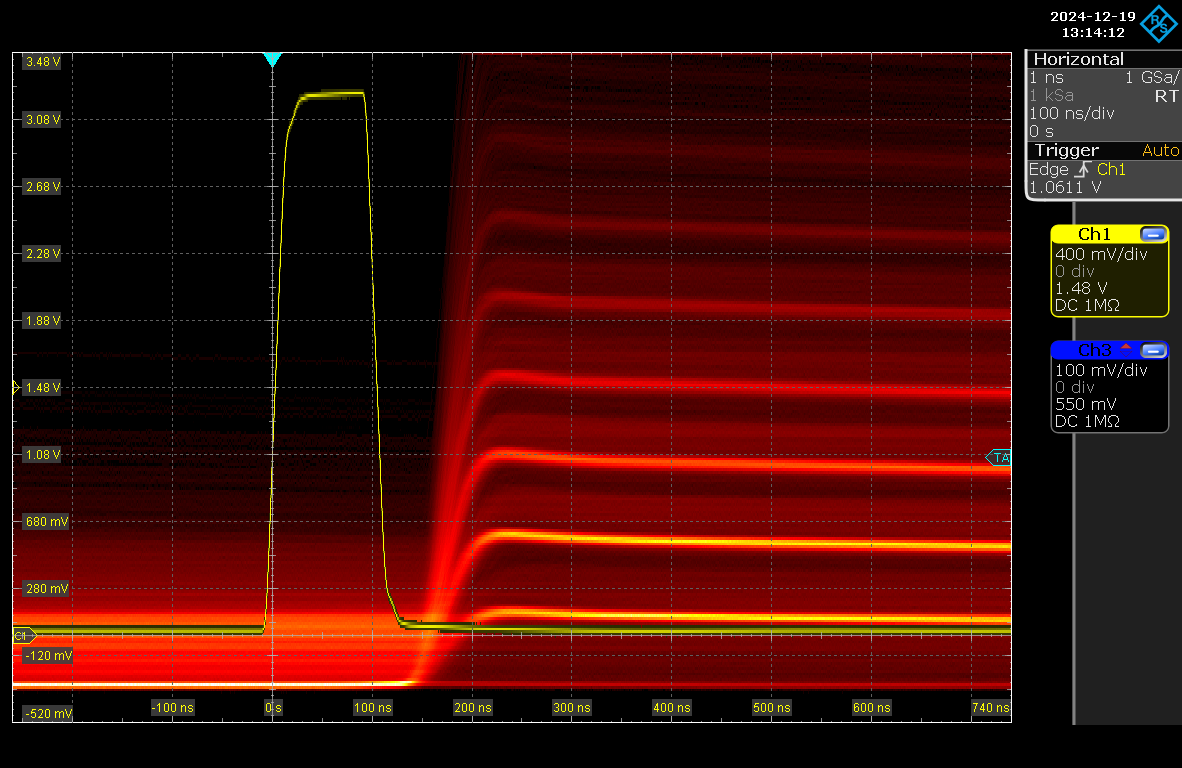
\includegraphics[width=0.5\linewidth]{Photomultiplier/assets/SiPm/SiPm.png}
    \caption{Prima visualizzazione dei segnali con persistance di 2 sec}
\end{figure}

E evidente la presenza di diverse zone con elevata densità di rilevazioni che corrispondono a un numero di fotoni crescente all'aumentare del voltaggio. Questo fenomeno è causato da 2 fotoni che arrivano in tempi molto ravvicinati e vengono rilevati come un unico evento.\\
Una volta collegato l'ADC e il comparatore all'uscita del Peak Hold, è stato possibile rilevare le onde:

\begin{figure}[!h]
    \centering
    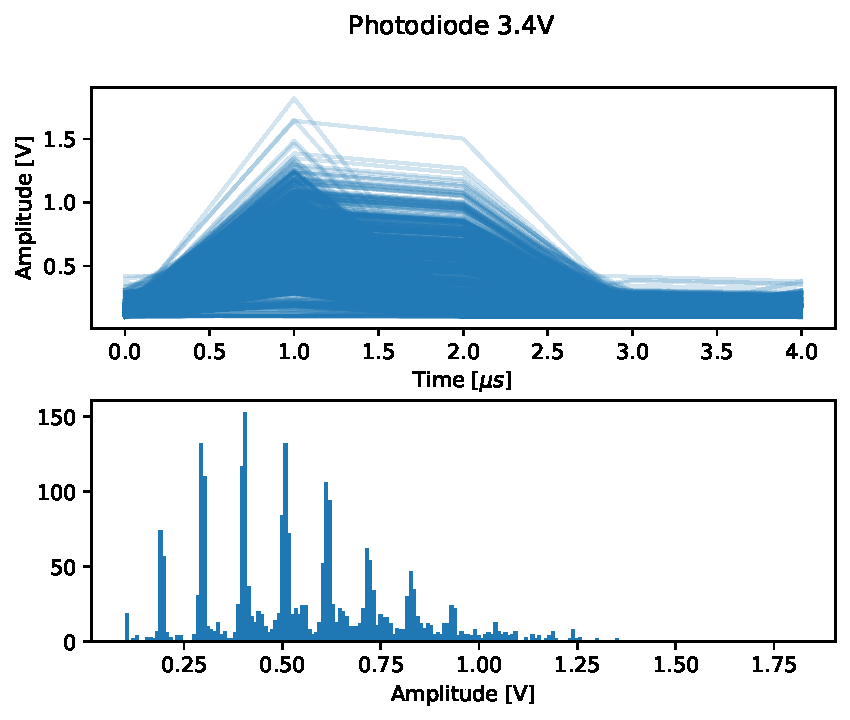
\includegraphics[width=0.5\linewidth]{Photomultiplier/assets/phot_3.4V.pdf}
    \caption{Segnale rilevato dall'ADC}
\end{figure}

Come si può notare, l'istogramma dei picchi è molto simile alla figura che si ha sull'oscilloscopio e i voltaggi sono molto simili.\\
Quello che ci aspettiamo è che i fotoni rilevati, siano tutti proporzionali alla misura del singolo fotone. Andando a calcolare i voltaggi che nell'istogramma corrispondevano ai picchi, siamo in grado di confrontare i valori ottenuti con i vari multipli del voltaggio di un singolo fotone.\\


\begin{wrapfigure}{r}{0.6\linewidth}
    \centering
    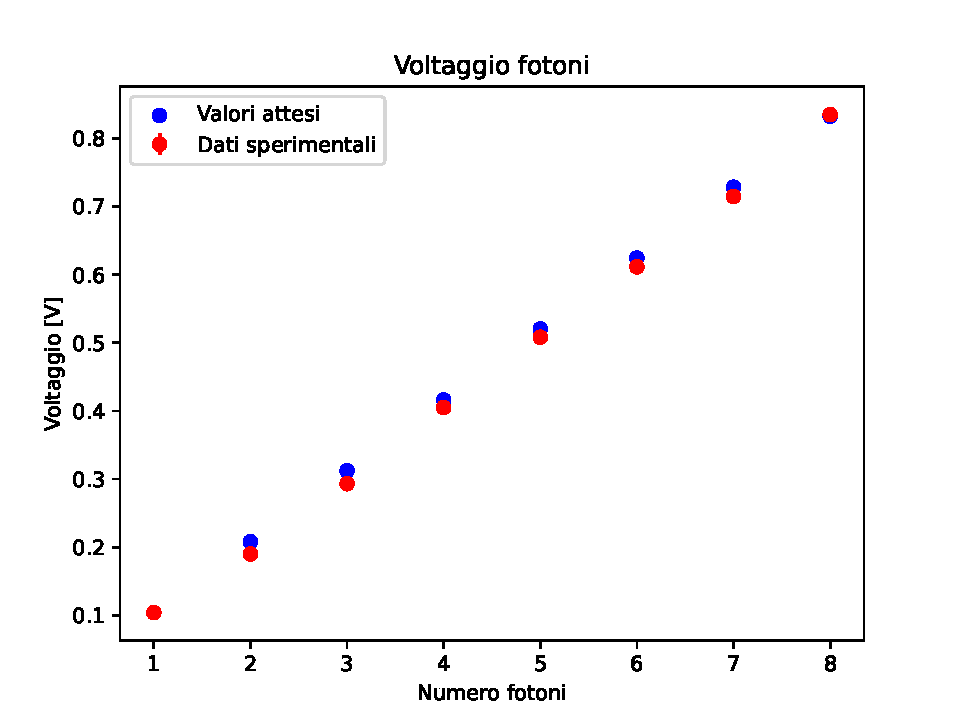
\includegraphics[width=\linewidth]{Photomultiplier/assets/Voltaggio_fotoni.pdf}
    \caption{Paragone tra dati ottenuti e valori aspettati}
    \label{fig:voltaggio_fotoni}
\end{wrapfigure}

Come si può vedere dall grafico \ref{fig:voltaggio_fotoni}, i valori ottenuti sono molto vicini ai valori attesi, e quindi confermare l'ipotesi.
Per quanto riguarda il rumore di sottofondo, si è notato che questo varia proporzionalmente a diversi fattori. In particolare, è proporzionale al voltaggio di alimentazione del fotomoltiplicatore. Questo è dovuto al fatto che il rumore di sottofondo è causato da elettroni che vengono emessi dal catodo e che vengono accelerati verso l'anodo. Aumentando il voltaggio di alimentazione, si aumenta la velocità degli elettroni e quindi la probabilità che questi vengano rilevati.\\

Come si può vedere dal grafico \ref{fig:dark_count}, gli istogrammi di Dark Count sono molto diversi con una differenza di solo $2V$ e questo è ragionevole pensare abbia un'influenza anche con il LED acceso.\\

Questa condizione motiva la presenza di più fotoni a tensioni più alte rispetto a quello che ci aspettavamo: ovvero di avere più misure di singolo fotone che altro.\\
\begin{wrapfigure}{l}{0.5\linewidth}
    \centering
    \includegraphics[width=\linewidth]{Photomultiplier/assets/Paragone_dark_count.pdf}
    \label{fig:dark_count}
\end{wrapfigure}